\documentclass[conference]{IEEEtran} 
\usepackage{graphicx}
\usepackage{amsmath}
\usepackage{alltt}
\usepackage{times}
\usepackage{url}

%% revisit the title.
\title{A dynamic loop pipelining mechanism for the efficient realization of algorithms as hardware}

\author{Madhav P. Desai\\
  Indian Institute of Technology -- Bombay, Powai, Mumbai -- 400076, INDIA\\
  Email: madhav@ee.iitb.ac.in }
\newtheorem{definition}{Definition}[section]
\newtheorem{theorem}{Theorem}[section]

\newcommand{\sym}[1]{$\operatorname{#1}$}

\pagestyle{empty}

\begin{document}

\maketitle
\thispagestyle{empty}

\begin{abstract}

  In the context of mapping high-level algorithms to hardware,
  we consider the basic problem of generating an efficient hardware 
  implementation of a loop.  We describe a control-flow mechanism through
  which multiple iterations of an arbitrary loop can be dynamically pipelined in
  the generated hardware,  and study the extent to which this 
  mechanism affects the properties of the generated hardware.
  We consider some common loop kernels occurring in fast-fourier transform,
  matrix multiplication and inner product computations, and
  observe that this dynamic pipelining mechanism typically results in
  a doubling of the performance of the hardware.  When 
  combined with static loop unrolling,  the performance improvement
  ranges from 6X to 20X across the loop kernels that we have studied.
  These optimizations do have a hardware overhead, however.  We characterize
  the performance/cost trade-off using an FPGA target, and find
  that the loop optimizations not only improve performance, but
  also the cost/performance ratio of the resulting hardware.

\end{abstract}

\section{Introduction}

%% The importance and problem of loops.
A high-level-synthesis (HLS) compiler takes an algorithm described in
a high-level programming language (such as C, for example) and produces a circuit
description (a register-transfer-level description in a hardware
description language such as VHDL, for example).
High-level synthesis systems have been available for some time
now (for example, \cite{pegasus-cash}, \cite{spark-vlsi-paper} and
commercial tools such as Catapult-C\footnote{\url{http://www.mentor.com/products/esl/high_level_synthesis/}} from Mentor Graphics
C-to-Silicon\footnote{\url{http://www.cadence.com/products/sd/silicon_compiler/}} from Cadence,
Synopsys HLS\footnote{\url{http://www.synopsys.com/Tools/SLD/HLS/}} from Synopsys).

The main attraction of such a compiler is a substantial reduction in 
the design and verification effort.  The
main concern is the quality of the hardware that is produced.
For the same starting point, the quality of the hardware produced may be objectively
measured in terms of factors such as area, energy-consumption and performance (in the
sense of time required for completion, or in terms of the rate at which the hardware
finishes the computational tasks).  An {\em internal measure} of the quality of the
hardware produced is the utilization factor of the major resources in the hardware (that is,
the utilization factor of expensive resources).  

%% How compilers have handled this problem.
In this paper, we consider the problem of mapping loops to hardware.  It
is well known that most compute intensive programs spend a large fraction
of their time in inner loops.  Thus, the optimization of these loops is
a primary problem for any optimizing compiler which is targetting
either a deeply pipelined or parallel processor.  Several loop optimizations
have been considered in literature, such as loop-unrolling, loop-peeling,
software-loop-pipelining etc. \cite{wolfe}, \cite{muchnick}, with the intent of
these optimizations being the extraction of as much
parallelism as possible from the source program. 

%% Algorithm-to-hardware:  can similar techniques work?
Several loop-optimization techniques have been explored and
reported in the literature related to reconfigurable hardware (for
example \cite{Weinhardt}, \cite{Cardoso}, \cite{Kastner}).  For instance,
in the work reported by \cite{Weinhardt},
the loop optimizations are done in a manner analogous to the static
techniques used in software compilers, in which index 
expressions which depend on the induction variable
are analysed to identify dependencies and schedule operations
in the loop body.  An explicitly timed controller is synthesized
for the pipeline.  Another approach which works in a similar
manner is described in \cite{Cardoso}.  These approaches rely on a static analysis of
the loop, and the cases to which the approach can be applied
are restricted (but still sufficiently general for most linear
algebra and digital signal processing kernels).


In our approach, the hardware model consists of a data-path (which is
a graph of operators interconnected by wires) and an untimed control-path
which is modeled as a Petri-net.  This representation allows the implementation
of loop pipelining by a simple modification to the control Petri-net
{\em without altering} the data-path.  Thus,
it is possible to pipeline any loop, even those that do not have 
explicit induction variables (such as while loops).  


The experimental results in this paper are based on the dynamic loop-pipelining
optimization applied by itself and in conjunction with static loop-unrolling.
By loop-unrolling, we mean a {\em static} compile-time optimization technique in
which   an inner loop is unrolled by instantiating multiple copies of the loop-body
while simultaneously reducing the number of loop-iterations.  For example:
\begin{verbatim}
for(i=0; i < 8; i++) {
   x += a[i]*b[i];
}
\end{verbatim}
is transformed to
\begin{verbatim}
for(i=0; i < 4; i+=2) {
   x += a[i]*b[i];
   x += a[i+1]*b[i+1];
}
\end{verbatim}
This unrolling increases the size of the basic block (that is, the maximal sequence of
statements without any branches), and provides the possibility of extracting more
parallelism in the loop.

In the remainder of this paper, we will first briefly describe the model of
the hardware that is produced by our HLS compiler and illustrate how this model
can incorporate dynamic run-time loop pipelining.  The chief issues here are the
hardware overhead (area, energy, delay) incurred by the need to provide 
this run-time support in the hardware generated by the compiler, and
the corresponding improvement in performance that results from this optimization.

In order to address this issue, we will present a set of observations from
experiments performed on representative inner loops that occur in 
some important applications such as the fast-fourier transform, the
matrix product, vector dot-product, and a digital filtering algorithm.
These observations report the hardware performance on four different
loop-optimization choices: with no loop optimization, with static unrolling
alone, with dynamic loop pipelining alone, and with static unrolling combined with
dynamic loop pipelining.  Hardware resource utilization and delays are
computed by synthesizing and simulating the generated hardware for an FPGA target.

The observations indicate the following:
\begin{itemize}
\item The performance improvement with loop-pipelining applied alone is in the
2X-3X range.
\item The performance improvement with loop-unrolling alone is in the 
2X range, and with aggressive unrolling (as was tried in the matrix multiplication
case), the improvement is as high as 10X.
\item The combination of loop-pipelining and loop-unrolling leads
to a performance improvement which is at least as high as the
product of the improvements due to the individual optimizations.  
For matrix multiplication, this improvement is as large as 20X.
\item The hardware overheads for implementing these optimizations are substantial,
but the cost-to-performance ratio improves substantially in all cases.
\end{itemize}


%%
%% TODO..  so what?
%% 

\section{A note on our compiler flow}

We give a brief description of our compiler flow.  The
details are not relevant to this paper, and the interested
reader can find them in \cite{dsd2010}.

Our compiler starts with a C program and produces VHDL.  For the
C front-end, we use the clang-2.8 compiler\footnote{www.clang.org}.
This compiler is used to emit LLVM byte-code\footnote{www.llvm.org}, 
which is then transformed to VHDL using the following transformations:
\begin{enumerate}
\item The LLVM byte-code is translated to an internal intermediate
format, which is itself a static-single assignment centric 
control-flow language (named {\bf Aa}) which allows the description of parallelism
using fork-join structures as well as arbitrary branching \cite{Aa}.
\item The {\bf Aa} description is translated to a virtual circuit (the model
is described in the next section).  During this translation, the
following major optimizations
are performed:  declared storage objects are partitioned into disjoint memory
spaces using pointer reference analysis, and dependency analysis is used to
generate appropriate sequencing of operations in order to maximize the 
parallelism.
\item The virtual circuit is then translated to VHDL.  At this point,
decisions about operator sharing are taken.  Concurrency analysis is
used if a shared hardware unit needs arbitration.  The generated
VHDL uses a pre-designed library of useful operators ranging from
multiplexors, arbiters to pipelined floating point arithmetic units.
\end{enumerate}

The compiler flow has been characterized over a wide variety
of applications \cite{dsd2010}.   The Click-to-NetFPGA tool-chain \cite{usenix2012} 
uses this compiler flow to map modular network appliances written in C++ to
an FPGA platform, and achieved about half the
performance possible using equivalent hand designed hardware.  
Thus,  the flow can be applied to ``real'' software
to produce competitive results.  The optimizations indicated in this
paper, should in principle, make the flow even more competitive.

%% compiler techniques.

%% hls techniques to handle loops?


\section{Model of hardware generated by our compiler}

The hardware generated by our compiler consists of three
cooperating components: the control-path, the data-path and
the storage system \cite{ahir}

To illustrate the model, we consider a simple example.
\begin{verbatim}
float a[1024], b[1024];
float dotp = 0.0;
for(i=0; i < 1024; i++)
{
   dotp += a[i]*b[i];
}
\end{verbatim}
To compile this code, we use the clang-2.8 \cite{clang} C compiler, 
which is used to emit LLVM \cite{llvm} byte-code.  The LLVM byte-code
is transformed through a series of steps by our compiler tools to
produce the final hardware, which is depicted in Figure \ref{fig:dotP}.
\begin{figure*}[ht]
  \centering
  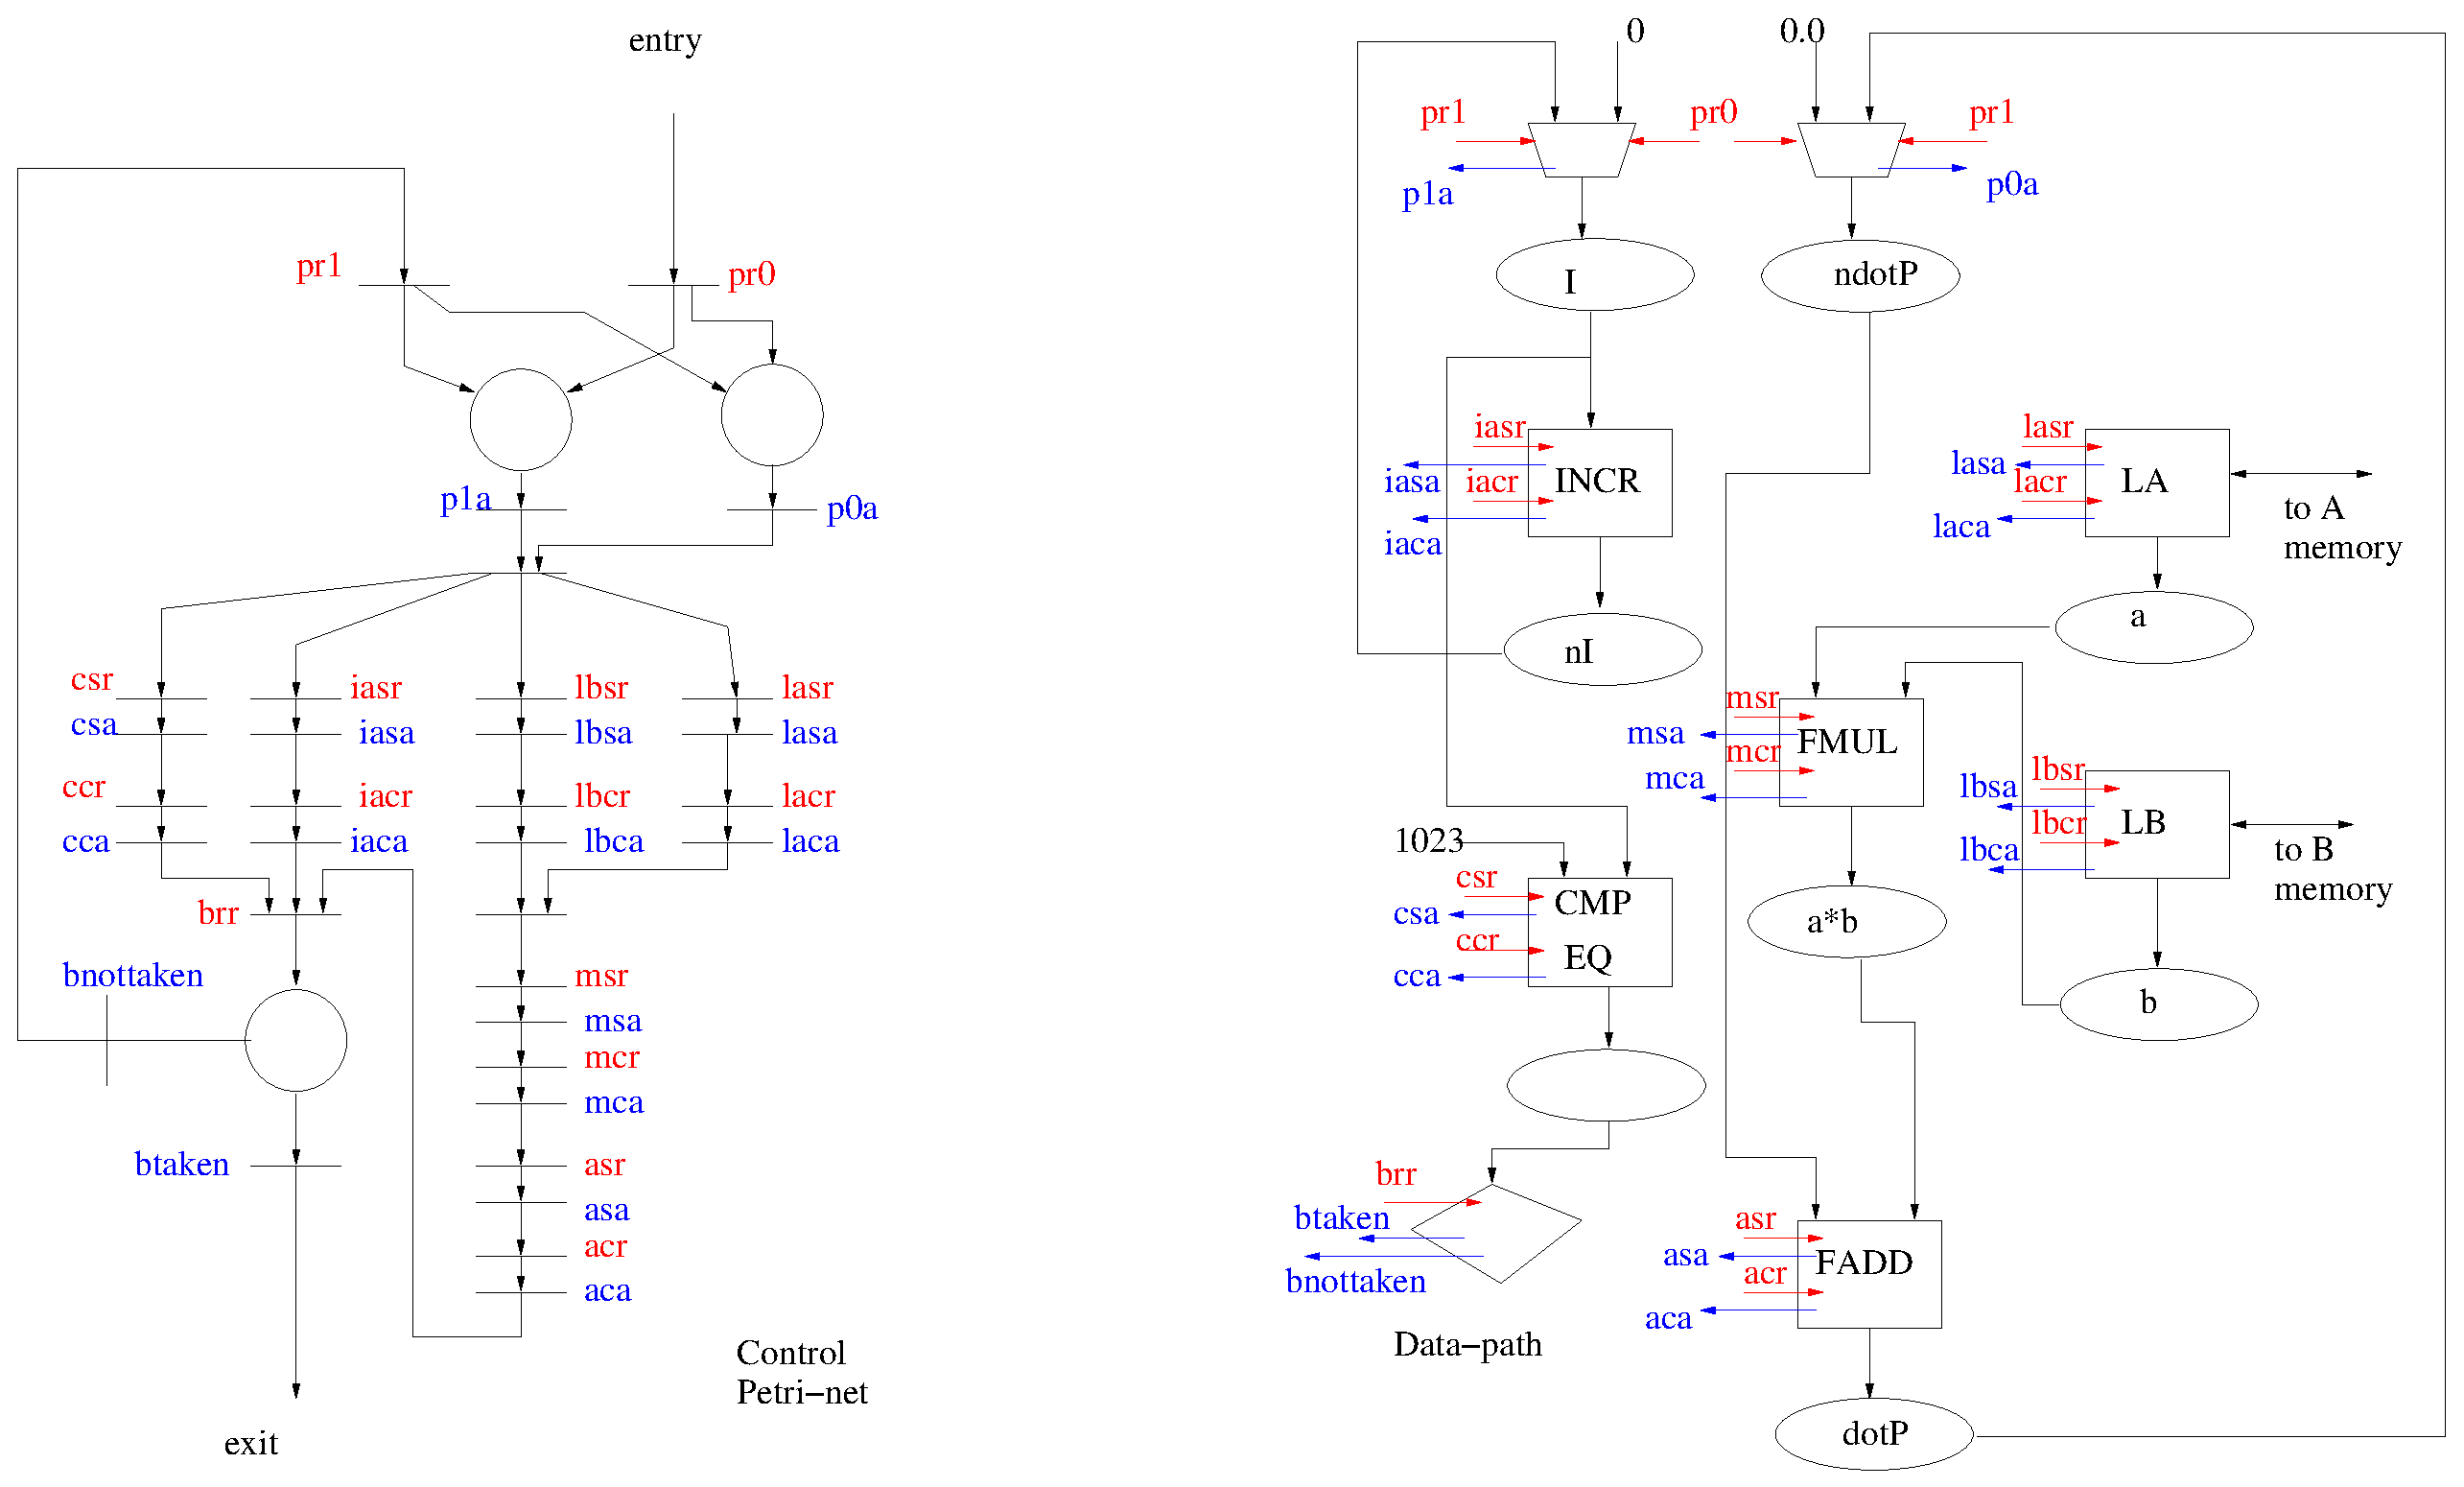
\includegraphics[width=15cm]{dotP.eps}
  \caption{Control-data-storage hardware model.}
  \label{fig:dotP}
\end{figure*}
The circuit in Figure \ref{fig:dotP} has three components,
described below.

\subsection{Control-path}
%%
%%  control path and data-flow
%%


%% 
%% Petri-net, constructed according to
%% certain rules.  Req/Ack transitions
%%
The hardware model consists of a control-path (shown on the left
in Figure \ref{fig:dotP}) which is modeled as a Petri-net with
a unique entry point and a unique exit point.  The Petri-net
is constructed using a set of production rules which guarantee
liveness and safeness \cite{ahir}.  Transitions in the Petri-net
are associated with output symbols to the data-path (these can
be described by the regular expressions *sr and *cr)
and input symbols from the data-path (these are of the form *sa and
*ca).  The *sr symbols instruct an element in the data-path to
sample its inputs and the *cr symbols instruct an element in the
data-path to update its outputs (all outputs of data-path elements
are registered).  The *sa and *ca symbols are acknowledgements
from the data-path which indicate that the corresponding requests
have been served.  


\subsection{Data-path}
%%
%% Directed hyper-graph.  Nodes are operators
%% hyper-arcs are wires.  Each operator node
%% has a split protocol.
%%
The data-path is a directed hyper-graph.  The operators
are shown as boxes and have input and output nets.  Each
net has at most one element which drives it.  Further, most
operators have  a split protocol handshake with
the control-path:  two pairs of request/acknowledge 
associations (*sr/*sa for sampling the inputs  and *cr/*ca for
updating the outputs).    The sequencing is required to be
\begin{verbatim}
sr -> sa -> cr -> ca
\end{verbatim}

Some data-path elements (such as the multiplexor
shown on the top and the decision operator shown at the bottom
left in Figure \ref{fig:dotP} follow a simpler protocol.  The multiplexor
has a pair of requests and a single acknowledge, with the condition
that at most one of the requests is received at any time instant.
The input corresponding to the request is then sampled and updates
the output of the multiplexor.
acknowledge lines.
The decision element has a single request and two acknowledes.  Upon
receipt of the request symbol, the decision element checks its input
and emits one of the two acknowledges depending on whether the input
is zero/non-zero.

In figure \ref{fig:dotP}, the following data-path elements
are instantiated:
\begin{verbatim}
mI, mdotP  multiplexors for I, dotP.
INCR       incrementor for I++
LA         load-operator for a[I]
LB         load-operator for b[I]
FMUL       multiplier for p=a[I]*b[I]
FADD       adder for dotP += a*b
CMP EQ     comparator COND=I==1023
D          decision  COND?
\end{verbatim}


\subsection{Storage subsystem}

%%
%% time-stamping scheme, in order completion.
%%
The load (and in general, store) operators in the data-path
are associated with memory subsystems.  In general, there
can be multiple disjoint memory subsystems inferred by our
compiler.  In this particular case, the array a[] and b[] 
are mapped to disjoint memories, due to which the two
loads are allowed to proceed in parallel (the relaxed consistency
model is enforced).
In order to maintain the relaxed consistency model, the
memory subsystems are designed to use a time-stamping 
scheme which guarantees first-come-first-served access to
the same memory location.

\subsection{Dependency analysis and extraction of parallelism}

Our compiler does a routine dependency analysis and enforces
the following dependencies between operations in the
data-path (these dependencies are enforced by the control-path):
\begin{itemize}
\item RAW: if the wire updated by operation A is used in an
operation B, the the sample-request to B is generated only
after the update-acknowledge from A.
\item WAR: if B writes to a wire which was earlier being read
by A (in the same loop iteration), then the update-request to B
can only be generated after the sample-acknowledge from A.
\item Load-Store ordering: A relaxed consistency model
is used.  If a load L follows a store S
and both are associated with the same memory subsystem, then
sample-start of the load L must begin after sample-acknowledge
of S (note that the memory subsystem maintains the service order).
Store-after-load and store-after-store dependencies are
handled in the same manner.  Successive loads without
an intervening store are allowed to finish in arbitrary order.
\end{itemize}

The control-path in \ref{fig:dotP} shows the sequencing
generated by these rules.  Note that the data-path
is not party to any sequencing decisions.  The data-path
elements must adhere to the request/acknowledge protocol
defined by the control-path.

\section{A control-flow mechanism for loop-pipelining}

%%
%% reenable rules.
%%
%% loop-terminator.
%%
%% advantages of dynamic pipelining: any loop
%% can be handled..
%%
Suppose that we want to modify the control-path in order to
permit the second (and maybe third etc.) iteration of a loop
to begin while the first iteration is still in progress.  
The 

\section{Experimental Results}

%%
%% examples: vector add, dot-product, matrix-multiply, linfinity-norm.
%%
%%
%%       show results without-unrolling-pipelining, with-unrolling-pipelining, etc.
%%

\section{Conclusion}

%%
%% loop-pipelining and loop-unrolling have high impact as
%% in pipelined processors.
%%
%% hardware mechanism for loop-pipelining is cheap and effective.
%%
%% can get 10X improvement and very high utilization of 
%% hardware resources.
%%

\bibliography{ref}
\bibliographystyle{IEEEtran}

\end{document}

% LocalWords:  Req Ack LL DP CP cmpgt br cdfg cp dp ir intra req init NCA SA mW
% LocalWords:  TPR STPR STPRs ccccc RTL ASIC petri ack versa liveness LRG LLVM
% LocalWords:  VHDL SRAM Synopsys AES LPK Linpack FFT RBT Synposys OSU TSMC nJ
% LocalWords:  nm
